% Options for packages loaded elsewhere
\PassOptionsToPackage{unicode}{hyperref}
\PassOptionsToPackage{hyphens}{url}
%
\documentclass[
]{article}
\usepackage{amsmath,amssymb}
\usepackage{iftex}
\ifPDFTeX
  \usepackage[T1]{fontenc}
  \usepackage[utf8]{inputenc}
  \usepackage{textcomp} % provide euro and other symbols
\else % if luatex or xetex
  \usepackage{unicode-math} % this also loads fontspec
  \defaultfontfeatures{Scale=MatchLowercase}
  \defaultfontfeatures[\rmfamily]{Ligatures=TeX,Scale=1}
\fi
\usepackage{lmodern}
\ifPDFTeX\else
  % xetex/luatex font selection
\fi
% Use upquote if available, for straight quotes in verbatim environments
\IfFileExists{upquote.sty}{\usepackage{upquote}}{}
\IfFileExists{microtype.sty}{% use microtype if available
  \usepackage[]{microtype}
  \UseMicrotypeSet[protrusion]{basicmath} % disable protrusion for tt fonts
}{}
\makeatletter
\@ifundefined{KOMAClassName}{% if non-KOMA class
  \IfFileExists{parskip.sty}{%
    \usepackage{parskip}
  }{% else
    \setlength{\parindent}{0pt}
    \setlength{\parskip}{6pt plus 2pt minus 1pt}}
}{% if KOMA class
  \KOMAoptions{parskip=half}}
\makeatother
\usepackage{xcolor}
\usepackage[margin=1in]{geometry}
\usepackage{color}
\usepackage{fancyvrb}
\newcommand{\VerbBar}{|}
\newcommand{\VERB}{\Verb[commandchars=\\\{\}]}
\DefineVerbatimEnvironment{Highlighting}{Verbatim}{commandchars=\\\{\}}
% Add ',fontsize=\small' for more characters per line
\usepackage{framed}
\definecolor{shadecolor}{RGB}{248,248,248}
\newenvironment{Shaded}{\begin{snugshade}}{\end{snugshade}}
\newcommand{\AlertTok}[1]{\textcolor[rgb]{0.94,0.16,0.16}{#1}}
\newcommand{\AnnotationTok}[1]{\textcolor[rgb]{0.56,0.35,0.01}{\textbf{\textit{#1}}}}
\newcommand{\AttributeTok}[1]{\textcolor[rgb]{0.13,0.29,0.53}{#1}}
\newcommand{\BaseNTok}[1]{\textcolor[rgb]{0.00,0.00,0.81}{#1}}
\newcommand{\BuiltInTok}[1]{#1}
\newcommand{\CharTok}[1]{\textcolor[rgb]{0.31,0.60,0.02}{#1}}
\newcommand{\CommentTok}[1]{\textcolor[rgb]{0.56,0.35,0.01}{\textit{#1}}}
\newcommand{\CommentVarTok}[1]{\textcolor[rgb]{0.56,0.35,0.01}{\textbf{\textit{#1}}}}
\newcommand{\ConstantTok}[1]{\textcolor[rgb]{0.56,0.35,0.01}{#1}}
\newcommand{\ControlFlowTok}[1]{\textcolor[rgb]{0.13,0.29,0.53}{\textbf{#1}}}
\newcommand{\DataTypeTok}[1]{\textcolor[rgb]{0.13,0.29,0.53}{#1}}
\newcommand{\DecValTok}[1]{\textcolor[rgb]{0.00,0.00,0.81}{#1}}
\newcommand{\DocumentationTok}[1]{\textcolor[rgb]{0.56,0.35,0.01}{\textbf{\textit{#1}}}}
\newcommand{\ErrorTok}[1]{\textcolor[rgb]{0.64,0.00,0.00}{\textbf{#1}}}
\newcommand{\ExtensionTok}[1]{#1}
\newcommand{\FloatTok}[1]{\textcolor[rgb]{0.00,0.00,0.81}{#1}}
\newcommand{\FunctionTok}[1]{\textcolor[rgb]{0.13,0.29,0.53}{\textbf{#1}}}
\newcommand{\ImportTok}[1]{#1}
\newcommand{\InformationTok}[1]{\textcolor[rgb]{0.56,0.35,0.01}{\textbf{\textit{#1}}}}
\newcommand{\KeywordTok}[1]{\textcolor[rgb]{0.13,0.29,0.53}{\textbf{#1}}}
\newcommand{\NormalTok}[1]{#1}
\newcommand{\OperatorTok}[1]{\textcolor[rgb]{0.81,0.36,0.00}{\textbf{#1}}}
\newcommand{\OtherTok}[1]{\textcolor[rgb]{0.56,0.35,0.01}{#1}}
\newcommand{\PreprocessorTok}[1]{\textcolor[rgb]{0.56,0.35,0.01}{\textit{#1}}}
\newcommand{\RegionMarkerTok}[1]{#1}
\newcommand{\SpecialCharTok}[1]{\textcolor[rgb]{0.81,0.36,0.00}{\textbf{#1}}}
\newcommand{\SpecialStringTok}[1]{\textcolor[rgb]{0.31,0.60,0.02}{#1}}
\newcommand{\StringTok}[1]{\textcolor[rgb]{0.31,0.60,0.02}{#1}}
\newcommand{\VariableTok}[1]{\textcolor[rgb]{0.00,0.00,0.00}{#1}}
\newcommand{\VerbatimStringTok}[1]{\textcolor[rgb]{0.31,0.60,0.02}{#1}}
\newcommand{\WarningTok}[1]{\textcolor[rgb]{0.56,0.35,0.01}{\textbf{\textit{#1}}}}
\usepackage{longtable,booktabs,array}
\usepackage{calc} % for calculating minipage widths
% Correct order of tables after \paragraph or \subparagraph
\usepackage{etoolbox}
\makeatletter
\patchcmd\longtable{\par}{\if@noskipsec\mbox{}\fi\par}{}{}
\makeatother
% Allow footnotes in longtable head/foot
\IfFileExists{footnotehyper.sty}{\usepackage{footnotehyper}}{\usepackage{footnote}}
\makesavenoteenv{longtable}
\usepackage{graphicx}
\makeatletter
\def\maxwidth{\ifdim\Gin@nat@width>\linewidth\linewidth\else\Gin@nat@width\fi}
\def\maxheight{\ifdim\Gin@nat@height>\textheight\textheight\else\Gin@nat@height\fi}
\makeatother
% Scale images if necessary, so that they will not overflow the page
% margins by default, and it is still possible to overwrite the defaults
% using explicit options in \includegraphics[width, height, ...]{}
\setkeys{Gin}{width=\maxwidth,height=\maxheight,keepaspectratio}
% Set default figure placement to htbp
\makeatletter
\def\fps@figure{htbp}
\makeatother
\setlength{\emergencystretch}{3em} % prevent overfull lines
\providecommand{\tightlist}{%
  \setlength{\itemsep}{0pt}\setlength{\parskip}{0pt}}
\setcounter{secnumdepth}{-\maxdimen} % remove section numbering
\ifLuaTeX
  \usepackage{selnolig}  % disable illegal ligatures
\fi
\IfFileExists{bookmark.sty}{\usepackage{bookmark}}{\usepackage{hyperref}}
\IfFileExists{xurl.sty}{\usepackage{xurl}}{} % add URL line breaks if available
\urlstyle{same}
\hypersetup{
  pdftitle={Gov 50 Final Project},
  pdfauthor={Lauren Cruickshank},
  hidelinks,
  pdfcreator={LaTeX via pandoc}}

\title{Gov 50 Final Project}
\author{Lauren Cruickshank}
\date{}

\begin{document}
\maketitle

{
\setcounter{tocdepth}{2}
\tableofcontents
}
\hypertarget{clink-image-for-2024-election-predictions}{%
\subsection{\texorpdfstring{\href{https://www.270towin.com/maps/biden-trump-2024-map-based-on-polls}{\protect\includegraphics{https://media-cldnry.s-nbcnews.com/image/upload/rockcms/2023-11/231106-Election-Preview-Joanna-Neborsky-jg-72121e.jpg}}}{Clink Image for 2024 Election Predictions}}\label{clink-image-for-2024-election-predictions}}

\hypertarget{code-chart}{%
\section{Code Chart}\label{code-chart}}

The data file for this study is~\texttt{fpd.csv}~and contains the
following variables:

\begin{longtable}[]{@{}
  >{\raggedright\arraybackslash}p{(\columnwidth - 2\tabcolsep) * \real{0.2840}}
  >{\raggedright\arraybackslash}p{(\columnwidth - 2\tabcolsep) * \real{0.7160}}@{}}
\toprule\noalign{}
\endhead
\bottomrule\noalign{}
\endlastfoot
\textbf{Name} & \textbf{Description} \\
\texttt{chamber} & whether the candidate is in the House or Senate \\
\texttt{candidate} & the names of candidate, party, and state \\
\texttt{selffunding} & how much money the candidate funded themselves \\
\texttt{collectedfunding} & how much money the candidate funded from
outside sources \\
\texttt{overallfunding} & the overall money the candidate received in
funding \\
\texttt{Percent\ Self-funded} & percent of funding the candidate funded
from themselves \\
\texttt{result} & whether or not the candidate won or loss the
election \\
\texttt{pervote} & share percentage of votes received by the
candidate \\
\end{longtable}

\hypertarget{introduction}{%
\section{Introduction}\label{introduction}}

\hypertarget{background}{%
\subsection{\texorpdfstring{\textbf{Background}}{Background}}\label{background}}

The 2024 presidential election cycle is currently approaching. As it is
known, there is a host of factors that can effect ones campaign run and
thus the results of the election. The U.S states government has formed
very specific rules around the use of campaign funds and the way that
they are used. Nonetheless, this study aims to find if there is a
correlation between the amount of campaign funds a candidate has and
their election results. The data set represents the campaign funding and
election results of House and Senate candidates from 2016 to 2020. The
explanatory variable in this study is is the amount of funding that each
candidate receives. The response variable or outcome is whether the
candidate saw success in the election.

\hypertarget{hypotheses}{%
\subsection{\texorpdfstring{\textbf{Hypotheses}}{Hypotheses}}\label{hypotheses}}

The Hypotheses of this Study are as follows:

\begin{enumerate}
\def\labelenumi{\arabic{enumi})}
\tightlist
\item
  As the \textbf{amount of available campaign funding increases} so will
  the \textbf{wins of the candidates increase}
\item
  As the \textbf{amount of available campaign funding increases} so will
  the \textbf{share percentage of votes received by candidates in the
  elections increase}
\end{enumerate}

\hypertarget{sec-running-code}{%
\section{Data Interest}\label{sec-running-code}}

\begin{Shaded}
\begin{Highlighting}[]
\FunctionTok{library}\NormalTok{(tidyverse)}
\FunctionTok{library}\NormalTok{(dplyr)}
\FunctionTok{library}\NormalTok{(readr)}
\FunctionTok{library}\NormalTok{(gapminder)}
\FunctionTok{library}\NormalTok{(infer)}
\FunctionTok{library}\NormalTok{(moderndive)}


\NormalTok{cand\_sp }\OtherTok{\textless{}{-}} \FunctionTok{read\_csv}\NormalTok{(}\StringTok{"fpd.csv"}\NormalTok{)}

\NormalTok{cand\_sp}
\end{Highlighting}
\end{Shaded}

The sample used is comprised of data compiled by the OpenSecrets the
``nation's premier research group tracking money in U.S politics and its
effect on elections and public policy. In this study, OpenSecret's data
on candidate spending and results from 2016 to 2020 were used. In order
to include the percentage share by which the candidate won or loss, it
had to be individually searched in the database of OpenSecret.

\hypertarget{data-links}{%
\subsection{Data Links:}\label{data-links}}

\href{https://www.opensecrets.org/elections-overview/top-self-funders?cycle=2016}{\textbf{OpenSecrets}}

The \textbf{independent variable} in this study is the \emph{amount of
money that each candidate has for campaign funding}. The
\textbf{dependent variable} is the \emph{share percentage of votes the
candidates receive} and \emph{the results that each candidate yielded
from the election}.

In order to identify a relationship between overall campaign funding,
share percentage of votes from election, and candidates results from the
election, this analysis is utilizing a correlation research design.

The graph below represents the top twenty candidatyes with the highest
campaign funding from 2016 to 2020.

\begin{Shaded}
\begin{Highlighting}[]
\FunctionTok{options}\NormalTok{(}\AttributeTok{scipen =} \DecValTok{999}\NormalTok{)}


\NormalTok{cand\_sp}\SpecialCharTok{|\textgreater{}}
  \FunctionTok{slice\_max}\NormalTok{(overallfunding, }\AttributeTok{n =} \DecValTok{20}\NormalTok{)}\SpecialCharTok{|\textgreater{}}
\FunctionTok{ggplot}\NormalTok{(}
       \AttributeTok{mapping =} \FunctionTok{aes}\NormalTok{(}\AttributeTok{x =}\NormalTok{ overallfunding, }\AttributeTok{y =} \FunctionTok{fct\_reorder}\NormalTok{(Candidate, overallfunding))) }\SpecialCharTok{+}
  \FunctionTok{geom\_col}\NormalTok{()}\SpecialCharTok{+}
  \FunctionTok{labs}\NormalTok{(}\AttributeTok{x =} \StringTok{"Overall Campaign Funding(k) "}\NormalTok{,}
       \AttributeTok{y =} \StringTok{"Candidates"}\NormalTok{,}
       \AttributeTok{title =} \StringTok{" Overall Campaign Funding of Candidates from 2016 to 2020"}\NormalTok{,}
       \AttributeTok{caption =} \StringTok{"note: all candidates are not displayed but only the twenty highest funded"}\NormalTok{)}
\end{Highlighting}
\end{Shaded}

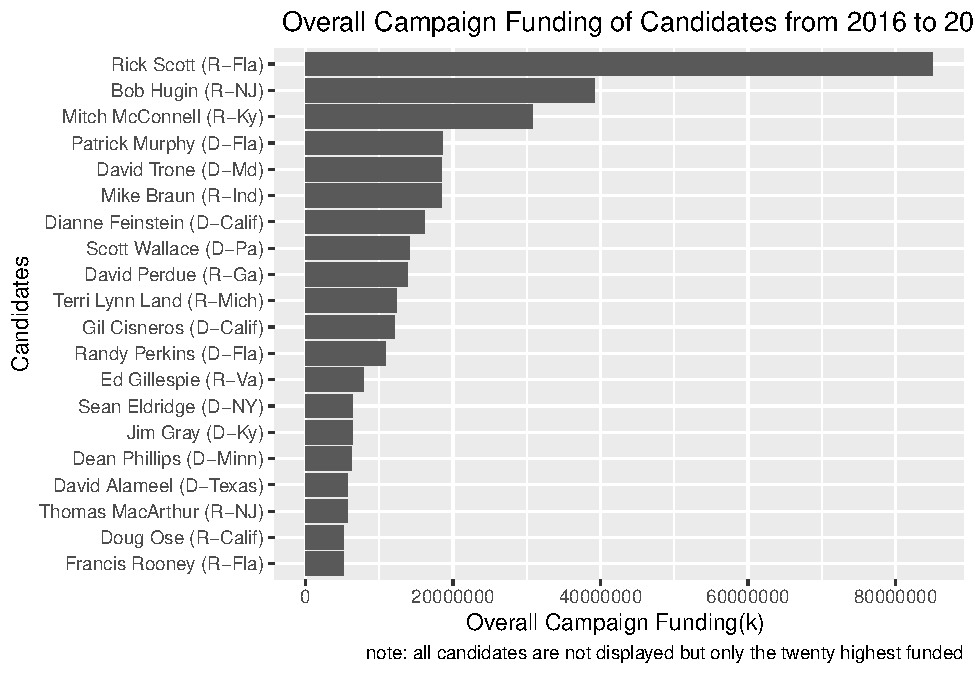
\includegraphics{index_files/figure-latex/unnamed-chunk-2-1.pdf}

\hypertarget{results}{%
\section{Results}\label{results}}

\hypertarget{linear-regression-between-the-share-of-votes-and-overall-funding-broken-down-by-loss-and-win}{%
\subsection{\texorpdfstring{\textbf{Linear Regression Between the Share
of Votes and Overall Funding Broken Down by Loss and
Win}}{Linear Regression Between the Share of Votes and Overall Funding Broken Down by Loss and Win}}\label{linear-regression-between-the-share-of-votes-and-overall-funding-broken-down-by-loss-and-win}}

The following multivariate regression model demonstrates the
relationship between the amount of money received for campaign funds,
the share percentage of votes the candidate received from the election,
and whether the candidate won or loss the overall election.

\begin{Shaded}
\begin{Highlighting}[]
\NormalTok{regr\_1 }\OtherTok{\textless{}{-}} \FunctionTok{lm}\NormalTok{(overallfunding }\SpecialCharTok{\textasciitilde{}}\NormalTok{ pervote }\SpecialCharTok{+}\NormalTok{ Result, }\AttributeTok{data =}\NormalTok{ cand\_sp)}
  
\NormalTok{ r1 }\OtherTok{\textless{}{-}} \FunctionTok{get\_regression\_table}\NormalTok{(regr\_1)}

\NormalTok{knitr}\SpecialCharTok{::}\FunctionTok{kable}\NormalTok{(}\FunctionTok{head}\NormalTok{(r1),}\AttributeTok{digits =} \DecValTok{2}\NormalTok{)}
\end{Highlighting}
\end{Shaded}

\begin{longtable}[]{@{}
  >{\raggedright\arraybackslash}p{(\columnwidth - 12\tabcolsep) * \real{0.1644}}
  >{\raggedleft\arraybackslash}p{(\columnwidth - 12\tabcolsep) * \real{0.1507}}
  >{\raggedleft\arraybackslash}p{(\columnwidth - 12\tabcolsep) * \real{0.1370}}
  >{\raggedleft\arraybackslash}p{(\columnwidth - 12\tabcolsep) * \real{0.1370}}
  >{\raggedleft\arraybackslash}p{(\columnwidth - 12\tabcolsep) * \real{0.1096}}
  >{\raggedleft\arraybackslash}p{(\columnwidth - 12\tabcolsep) * \real{0.1507}}
  >{\raggedleft\arraybackslash}p{(\columnwidth - 12\tabcolsep) * \real{0.1507}}@{}}
\toprule\noalign{}
\begin{minipage}[b]{\linewidth}\raggedright
term
\end{minipage} & \begin{minipage}[b]{\linewidth}\raggedleft
estimate
\end{minipage} & \begin{minipage}[b]{\linewidth}\raggedleft
std\_error
\end{minipage} & \begin{minipage}[b]{\linewidth}\raggedleft
statistic
\end{minipage} & \begin{minipage}[b]{\linewidth}\raggedleft
p\_value
\end{minipage} & \begin{minipage}[b]{\linewidth}\raggedleft
lower\_ci
\end{minipage} & \begin{minipage}[b]{\linewidth}\raggedleft
upper\_ci
\end{minipage} \\
\midrule\noalign{}
\endhead
\bottomrule\noalign{}
\endlastfoot
intercept & 2509749.46 & 5177210 & 0.48 & 0.63 & -7899729.1 &
12919228.0 \\
pervote & 87475.74 & 125817 & 0.70 & 0.49 & -165496.2 & 340447.7 \\
Result: Won & 6217351.12 & 4271917 & 1.46 & 0.15 & -2371913.3 &
14806615.5 \\
\end{longtable}

\hypertarget{interpretation}{%
\subsubsection{\texorpdfstring{\textbf{Interpretation}}{Interpretation}}\label{interpretation}}

The intercept of 2.509,749.46 , is the estimated campaign funding when
the share percentage of votes received by the candidate is zero and the
candidate did not win the election. There is an expected increase of
87,475.74 in campaign funding for each unit increase in the share
percentage of votes received by the candidate , also assuming that the
candidate winning status stays constant.

The coefficient for `Result: Won' of 6,217,351.12, shows that when a
candidate wins the election, there is an expected increase of
6,217,351.12 in campaign funds in comparison ton when the candidate does
not win, also assuming that the share percentage of votes stays
constant.

\begin{Shaded}
\begin{Highlighting}[]
\NormalTok{cand\_sp}\SpecialCharTok{|\textgreater{}}
  \FunctionTok{ggplot}\NormalTok{(}
    \AttributeTok{mapping =} \FunctionTok{aes}\NormalTok{(}
      \AttributeTok{x =}\NormalTok{ overallfunding,}
      \AttributeTok{y =}\NormalTok{ pervote,}
      \AttributeTok{color =}\NormalTok{ Result))}\SpecialCharTok{+}
  \FunctionTok{geom\_point}\NormalTok{()}\SpecialCharTok{+}
  \FunctionTok{geom\_smooth}\NormalTok{()}\SpecialCharTok{+}
  \FunctionTok{scale\_x\_log10}\NormalTok{()}\SpecialCharTok{+}
   \FunctionTok{labs}\NormalTok{(}\AttributeTok{x =} \StringTok{"Overall Campaign Funding(k) "}\NormalTok{,}
       \AttributeTok{y =} \StringTok{"Share Percentage Of Vote (\%)"}\NormalTok{,}
       \AttributeTok{title =} \StringTok{" Share Percentage of Vote vs. Campaign Funding (with Result)"}\NormalTok{)}
\end{Highlighting}
\end{Shaded}

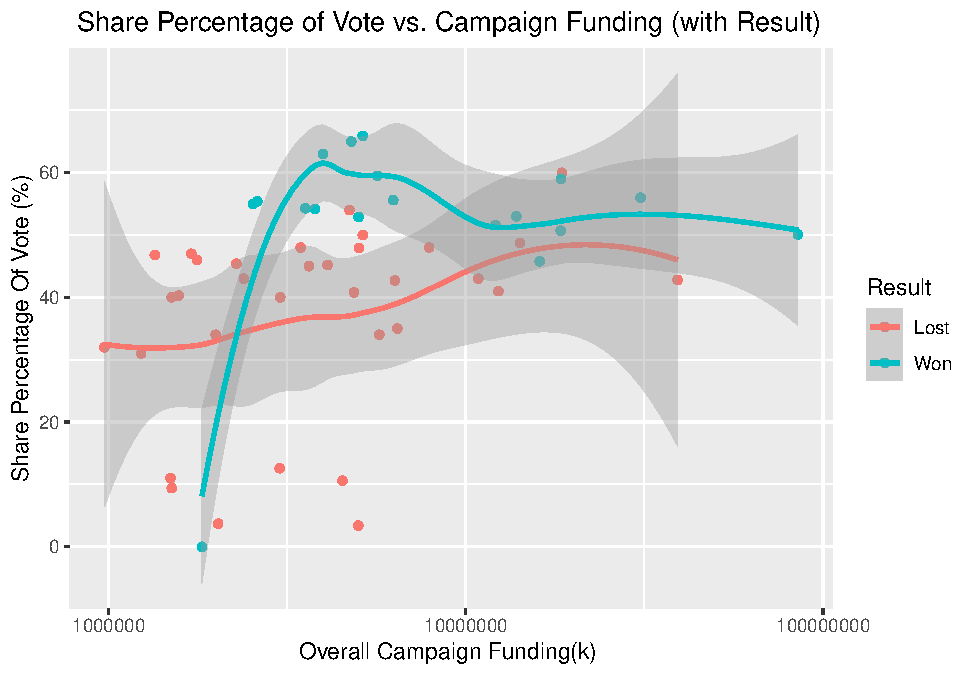
\includegraphics{index_files/figure-latex/unnamed-chunk-4-1.pdf}

The graph above suggest that with both losses and wins there is a slight
relationship between an increase of money and an increase of that
result. Within the graph it is also evident that candidates who lost
their elections experienced more variability in campaign funding than
those who won.

\hypertarget{linear-regression-between-the-share-of-votes-and-overall-funding}{%
\subsection{\texorpdfstring{\textbf{Linear Regression between the Share
of Votes and Overall
Funding}}{Linear Regression between the Share of Votes and Overall Funding}}\label{linear-regression-between-the-share-of-votes-and-overall-funding}}

\begin{Shaded}
\begin{Highlighting}[]
\NormalTok{null\_dist }\OtherTok{\textless{}{-}}\NormalTok{ cand\_sp }\SpecialCharTok{|\textgreater{}}
  \FunctionTok{specify}\NormalTok{(overallfunding }\SpecialCharTok{\textasciitilde{}}\NormalTok{ pervote) }\SpecialCharTok{|\textgreater{}}
  \FunctionTok{hypothesize}\NormalTok{(}\AttributeTok{null =} \StringTok{"independence"}\NormalTok{) }\SpecialCharTok{|\textgreater{}}
  \FunctionTok{generate}\NormalTok{(}\AttributeTok{reps =} \DecValTok{1000}\NormalTok{, }\AttributeTok{type =} \StringTok{"permute"}\NormalTok{) }\SpecialCharTok{|\textgreater{}}
  \FunctionTok{calculate}\NormalTok{(}\AttributeTok{stat =} \StringTok{"correlation"}\NormalTok{)}

\NormalTok{correlation }\OtherTok{\textless{}{-}}\NormalTok{ cand\_sp }\SpecialCharTok{|\textgreater{}}
  \FunctionTok{specify}\NormalTok{(overallfunding }\SpecialCharTok{\textasciitilde{}}\NormalTok{ pervote) }\SpecialCharTok{|\textgreater{}}
  \FunctionTok{calculate}\NormalTok{(}\AttributeTok{stat =} \StringTok{"correlation"}\NormalTok{)}

\NormalTok{null\_dist }\SpecialCharTok{|\textgreater{}}
  \FunctionTok{visualize}\NormalTok{() }\SpecialCharTok{+}
  \FunctionTok{shade\_p\_value}\NormalTok{(correlation, }\AttributeTok{direction =} \StringTok{"both"}\NormalTok{)}
\end{Highlighting}
\end{Shaded}

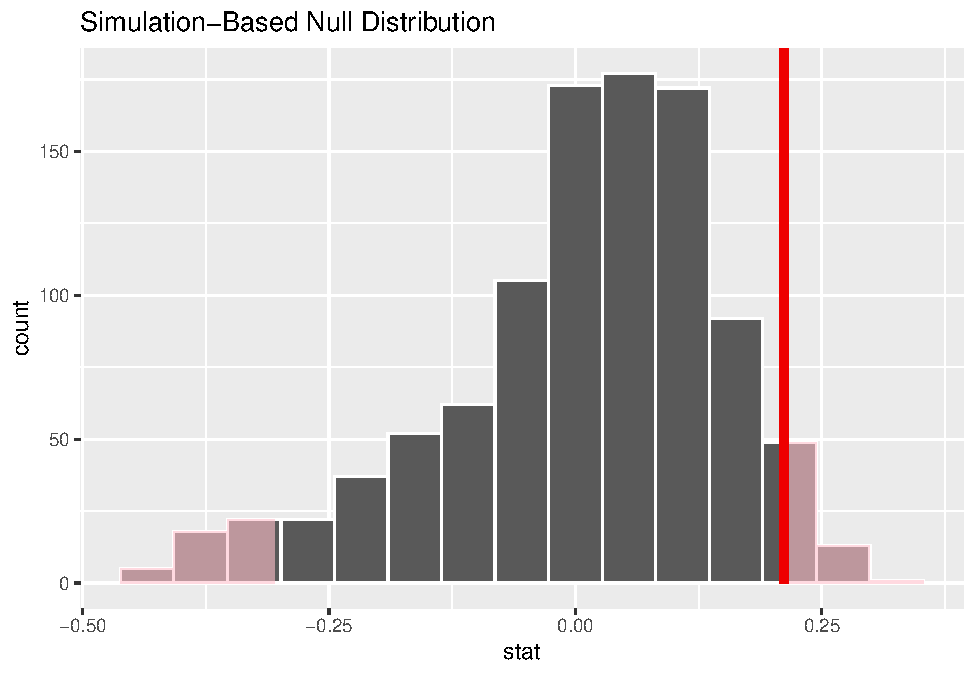
\includegraphics{index_files/figure-latex/unnamed-chunk-5-1.pdf}

\begin{Shaded}
\begin{Highlighting}[]
\FunctionTok{get\_p\_value}\NormalTok{(null\_dist, correlation, }\AttributeTok{direction =} \StringTok{"both"}\NormalTok{)}
\end{Highlighting}
\end{Shaded}

In this study, the null hypothesis suggest that there is no relationship
between the amount of campaign funding a candidate received and the
share percentage of votes they received in the election. With a
significance level of ⍺ = 0.05, we would fail to reject the null
hypothesis with a p-value of 0.072. Therefore, we conclude that there is
not a statistically significant relationship between campaign funds and
the share percentage of votes candidates receive in elections.

The following regression displays the relationship between the the
amount of funding a candidate received and the share percentage of votes
they received during the election process.

\begin{Shaded}
\begin{Highlighting}[]
\NormalTok{regr\_2 }\OtherTok{\textless{}{-}} \FunctionTok{lm}\NormalTok{(overallfunding }\SpecialCharTok{\textasciitilde{}}\NormalTok{ pervote, }\AttributeTok{data =}\NormalTok{ cand\_sp)}

\NormalTok{r2 }\OtherTok{\textless{}{-}} \FunctionTok{get\_regression\_table}\NormalTok{(regr\_2)}

\NormalTok{knitr}\SpecialCharTok{::}\FunctionTok{kable}\NormalTok{(}\FunctionTok{head}\NormalTok{(r2),}\AttributeTok{digits =} \DecValTok{2}\NormalTok{)}
\end{Highlighting}
\end{Shaded}

\begin{longtable}[]{@{}
  >{\raggedright\arraybackslash}p{(\columnwidth - 12\tabcolsep) * \real{0.1408}}
  >{\raggedleft\arraybackslash}p{(\columnwidth - 12\tabcolsep) * \real{0.1408}}
  >{\raggedleft\arraybackslash}p{(\columnwidth - 12\tabcolsep) * \real{0.1408}}
  >{\raggedleft\arraybackslash}p{(\columnwidth - 12\tabcolsep) * \real{0.1408}}
  >{\raggedleft\arraybackslash}p{(\columnwidth - 12\tabcolsep) * \real{0.1127}}
  >{\raggedleft\arraybackslash}p{(\columnwidth - 12\tabcolsep) * \real{0.1690}}
  >{\raggedleft\arraybackslash}p{(\columnwidth - 12\tabcolsep) * \real{0.1549}}@{}}
\toprule\noalign{}
\begin{minipage}[b]{\linewidth}\raggedright
term
\end{minipage} & \begin{minipage}[b]{\linewidth}\raggedleft
estimate
\end{minipage} & \begin{minipage}[b]{\linewidth}\raggedleft
std\_error
\end{minipage} & \begin{minipage}[b]{\linewidth}\raggedleft
statistic
\end{minipage} & \begin{minipage}[b]{\linewidth}\raggedleft
p\_value
\end{minipage} & \begin{minipage}[b]{\linewidth}\raggedleft
lower\_ci
\end{minipage} & \begin{minipage}[b]{\linewidth}\raggedleft
upper\_ci
\end{minipage} \\
\midrule\noalign{}
\endhead
\bottomrule\noalign{}
\endlastfoot
intercept & 1132003.8 & 5147677.4 & 0.22 & 0.83 & -9212641.27 &
11476648.8 \\
pervote & 171455.5 & 113073.6 & 1.52 & 0.14 & -55774.31 & 398685.3 \\
\end{longtable}

\hypertarget{interpretation-1}{%
\subsubsection{\texorpdfstring{\textbf{Interpretation}}{Interpretation}}\label{interpretation-1}}

The intercept of 1,132,003.8 , is the estimated campaign funding when
the share percentage of votes received by the candidate is zero. There
is an expected increase of 171,455.5 in campaign funding for each unit
increase in the share percentage of votes received by the candidate.

\begin{Shaded}
\begin{Highlighting}[]
\NormalTok{cand\_sp}\SpecialCharTok{|\textgreater{}}
  \FunctionTok{ggplot}\NormalTok{(}
    \AttributeTok{mapping =} \FunctionTok{aes}\NormalTok{(}
      \AttributeTok{x =}\NormalTok{ overallfunding,}
      \AttributeTok{y =}\NormalTok{ pervote))}\SpecialCharTok{+}
  \FunctionTok{geom\_point}\NormalTok{(}\AttributeTok{color =} \StringTok{"blue"}\NormalTok{)}\SpecialCharTok{+}
  \FunctionTok{geom\_smooth}\NormalTok{(}\AttributeTok{color =} \StringTok{"red"}\NormalTok{)}\SpecialCharTok{+}
  \FunctionTok{scale\_x\_log10}\NormalTok{()}\SpecialCharTok{+}
  \FunctionTok{labs}\NormalTok{(}\AttributeTok{x =} \StringTok{"Overall Campaign Funding(k) "}\NormalTok{,}
       \AttributeTok{y =} \StringTok{"Share Percentage Of Vote (\%)"}\NormalTok{,}
       \AttributeTok{title =} \StringTok{" Share Percentage of Vote vs. Campaign Funding"}\NormalTok{)}
\end{Highlighting}
\end{Shaded}

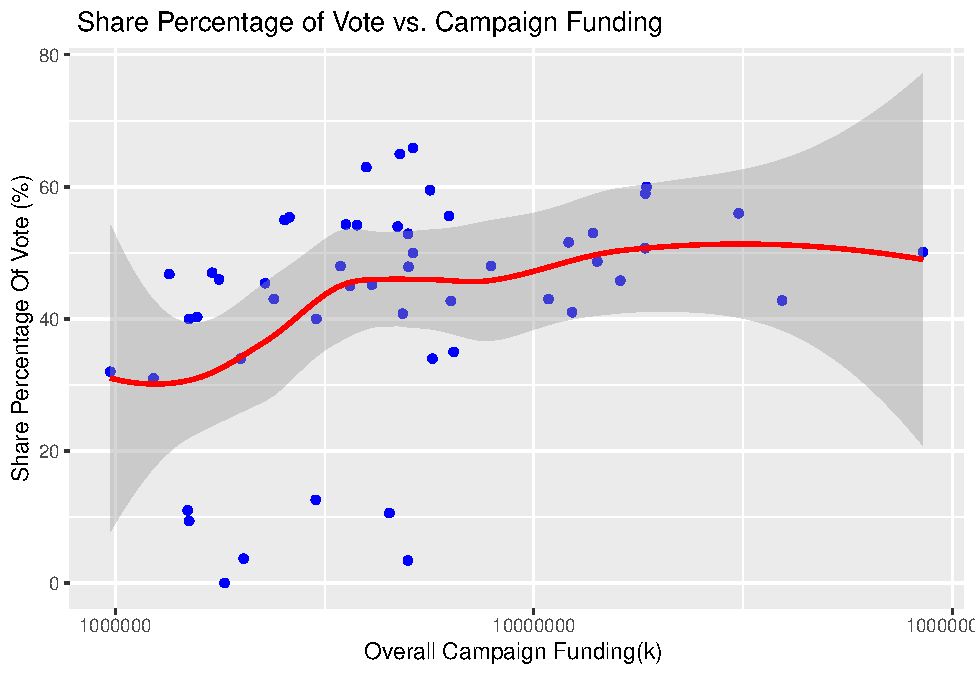
\includegraphics{index_files/figure-latex/unnamed-chunk-8-1.pdf}

The graph above denotes the relationship between the amount of campaign
funding a candidate has and the share percentage of votes they received
in the election. In this case, without evaluating which candidates won
or loss, there seems to be a \emph{slight positive correlation} between
an increase in funding and an increase in the share percentage of votes
the candidate received.

\hypertarget{conclusion}{%
\section{\texorpdfstring{\textbf{Conclusion}}{Conclusion}}\label{conclusion}}

From the findings above it is clear that that there is not a
statistically significant relationship between campaign funds and the
share percentage of votes candidates receive in elections. This can be
seen in the p-value of \texttt{pervote} at .14 which we would fail to
reject the null at the significance level of ⍺ of 0.05.

There is also not a statisitcally significant relationship between
campaign funds, the results of the campaign, and the share percentage of
votes candidates receive in elections. This can be seen by both the
p-value of 0.072 at a significance level ⍺ of 0.05 and with the
scatterplot of both loss and wins as the both have slight positive
relationships with the increase of campaign funding.

(talk about my hypothesis.

\textbf{Limitations}

It should be noted that this study only only considers monetary funding
as the main independent variable and thus the variable that is causing
the outcomes. However, in governmental elections that are a host of
factors that actually effect why a candidate may or may not be able to
secure the seat. There were also candidates that had to be removed from
the original data set because they were included in the main data frame
but may have not made it to the main election.

\textbf{Future Improvements}

In future studies more factors can be evaluated that are related to the
outcome of elections. They could possibly introduce how many commercials
a candidate used or polls that evaluate public opinion around how
candidates do in debates. With the introduction of more factors, the
causal reasoning of the study will be much stronger because there will
be less confounding variables.

\end{document}
